\subsection{Transformer:}

After rectified the signal, we assembly the circuit of the Figure 3.1.0, the transformer to be used it's of {\bfseries\itshape 12$V_{rms}$ to 1A} this means that in the {\bfseries\itshape secondary winding} the voltage will be approximately of 12$V_{rms}$. The {\bfseries\itshape primary winding} will be connected to the outlet plug and the voltage that will be driving will be approximately of 117$V_{rms}$. \hfill \break

We are going to be switching between two resistors: One of 100$\Omega$ at 10W and the other one of 22$\Omega$ at 25W. For each resistor, the voltage will be measured, and the result its going to be registered in the table bellow. \hfill \break

\begin{multicols}{2}
\begin{figure}[H]
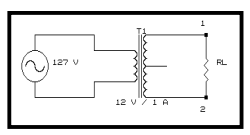
\includegraphics[scale=.8]{transformer.png}
\centering \linebreak \linebreak Figure 3.1.0: Transformer circuit.
\end{figure}

{\Large
\begin{center}
\begin{tabular}[.5cm]{l c c }
\toprule
$R_{L}$ & $V_{rms}$ \\
\midrule
100$\Omega$ & 13.2$V_{rms}$ \\
\cmidrule{1-2}
22$\Omega$ & 12.1$V_{rms}$ \\
\bottomrule
\linebreak
\end{tabular}
\end{center} }
    Table 1: Measured values of Figure 3.1.0.
\end{multicols}